\documentclass[xcolor=pdflatex,dvipsnames,table]{beamer}
\usepackage{epsfig,graphicx}
\usepackage{palatino}
\usepackage{fancybox}
\usepackage{relsize}
\usepackage[procnames]{listings}
\usepackage{hyperref}
\usepackage{qtree} % needed?
\usepackage{booktabs}
\usepackage{dirtree}
\usepackage[normalem]{ulem}


% fatter TT font
\renewcommand*\ttdefault{txtt}
% another TT, suggested by Alex
% \usepackage{inconsolata}
% \usepackage[T1]{fontenc} % needed as well?


\newcommand{\scale}{0.7}

\newcommand{\todo}[1]{{\emph{TODO: #1}}}
\newcommand{\martin}[1]{{\color{blue} Martin: #1}}
\newcommand{\abcdef}[1]{{\color{red} Author2: #1}}

% uncomment following for final submission
%\renewcommand{\todo}[1]{}
%\renewcommand{\martin}[1]{}
%\renewcommand{\author2}[1]{}

\newcommand{\code}[1]{{\texttt{#1}}}

\hypersetup{
  linkcolor  = black,
%  citecolor  = blue,
  urlcolor   = blue,
  colorlinks = true,
}

\beamertemplatenavigationsymbolsempty
\setbeamertemplate{footline}[frame number]





\newif\ifbook
% shared in slides and book

\lstdefinelanguage{chisel}{
%  morekeywords={abstract,case,catch,class,def,%
%    do,else,extends,false,final,finally,%
%    for,if,implicit,import,match,mixin,%
%    new,null,object,override,package,%
%    private,protected,requires,return,sealed,%
%    super,this,throw,trait,true,try,%
%    type,val,var,while,with,yield},
%  otherkeywords={=>,<-,<\%,<:,>:,\#,@},
  sensitive=true,
  morecomment=[l]{//},
  morecomment=[n]{/*}{*/},
  morestring=[b]",
  morestring=[b]',
  morestring=[b]"""
}

\usepackage{color}
\definecolor{dkgreen}{rgb}{0,0.6,0}
\definecolor{gray}{rgb}{0.5,0.5,0.5}
\definecolor{mauve}{rgb}{0.58,0,0.82}

% Default settings for code listings
%\ifbook
\lstset{%frame=lines,
  language=chisel,
  aboveskip=3mm,
  belowskip=3mm,
  showstringspaces=false,
  columns=fixed, % basewidth=\mybasewidth,
  basicstyle={\small\ttfamily},
  numbers=none,
  numberstyle=\footnotesize,
  % identifierstyle=\color{red},
  breaklines=true,
  breakatwhitespace=true,
  procnamekeys={def, val, var, class, trait, object, extends},
  % procnamestyle=\ttfamily,
  tabsize=2,
  float
}
%\else
%\lstset{%frame=lines,
%  language=chisel,
%  aboveskip=3mm,
%  belowskip=3mm,
%  showstringspaces=false,
%  columns=fixed, % basewidth=\mybasewidth,
%  basicstyle={\small\ttfamily},
%  numbers=none,
%  numberstyle=\footnotesize\color{gray},
%  % identifierstyle=\color{red},
%  keywordstyle=\color{blue},
%  commentstyle=\color{dkgreen},
%  stringstyle=\color{mauve},
%  breaklines=true,
%  breakatwhitespace=true,
%  procnamekeys={def, val, var, class, trait, object, extends},
%  procnamestyle=\ttfamily\color{red},
%  tabsize=2,
%  float
%}
%\fi

\lstnewenvironment{chisel}[1][]
{\lstset{language=chisel,#1}}
{}

\newcommand{\shortlist}[1]{{\lstinputlisting[nolol]{#1}}}

\newcommand{\longlist}[3]{{\lstinputlisting[float, caption={#2}, label={#3}, frame=tb, captionpos=b]{#1}}}

\newcommand{\verylonglist}[3]{{\lstinputlisting[caption={#2}, label={#3}, frame=tb, captionpos=b]{#1}}}



\title{Customized Circuit Generation}
\author{Martin Schoeberl}
\date{\today}
\institute{Technical University of Denmark}

\begin{document}

\begin{frame}
\titlepage
\end{frame}





\begin{frame}[fragile]{Scala List for Enumeration}
\begin{chisel}
  val empty :: full :: Nil = Enum(2)
\end{chisel}
\begin{itemize}
\item Can be used in wires and registers
\item Symbols for a state machine
\end{itemize}
\end{frame}

\begin{frame}[fragile]{Finite State Machine}
\begin{chisel}
  val empty :: full :: Nil = Enum(2)
  val stateReg = RegInit(empty)
  val dataReg = RegInit(0.U(size.W))

  when(stateReg === empty) {
    when(io.enq.write) {
      stateReg := full
      dataReg := io.enq.din
    }
  }.elsewhen(stateReg === full) {
    when(io.deq.read) {
      stateReg := empty
    }
  }
\end{chisel}
\begin{itemize}
\item A simple buffer for a bubble FIFO
\end{itemize}
\end{frame}

\begin{frame}[fragile]{Parameterization}
\begin{chisel}
class ParamChannel(n: Int) extends Bundle {
  val data = Input(UInt(n.W))
  val ready = Output(Bool())
  val valid = Input(Bool())
}

val ch32 = new ParamChannel(32)
\end{chisel}
\begin{itemize}
\item Bundles and modules can be parametrized
\item Pass a parameter in the constructor
\end{itemize}

\end{frame}
\begin{frame}[fragile]{A Module with a Parameter}
\begin{chisel}
class ParamAdder(n: Int) extends Module {
  val io = IO(new Bundle {
    val a = Input(UInt(n.W))
    val b = Input(UInt(n.W))
    val result = Output(UInt(n.W))
  })

  val addVal = io.a + io.b
  io.result := addVal
}

val add8 = Module(new ParamAdder(8))
\end{chisel}
\begin{itemize}
\item Parameter can also be a Chisel type
\item Can also be a generic type:
\item \code{class Mod[T <: Bits](param: T) extends...}
\end{itemize}
\end{frame}

\begin{frame}[fragile]{Scala \code{for} Loop for Circuit Generation}
\begin{chisel}
val shiftReg = RegInit(0.U(8.W))

shiftReg(0) := inVal

for (i <- 1 until 8) {
  shiftReg(i) := shiftReg(i-1)
}
\end{chisel}
\begin{itemize}
\item \code{for} is Scala
\item This loop generates several connections
\item The connections are parallel hardware
\end{itemize}
\end{frame}

\begin{frame}[fragile]{Conditional Circuit Generation}
\begin{chisel}
class Base extends Module { val io = new Bundle() }
class VariantA extends Base { }
class VariantB extends Base { }

val m = if (useA) Module(new VariantA())
        else Module(new VariantB())
\end{chisel}
\begin{itemize}
\item \code{if} and \code{else} is Scala
\item \code{if} is an expression that returns a value
\begin{itemize}
\item Like ``\code{cond ? a : b;}'' in C and Java
\end{itemize}
\item This is not a hardware multiplexer
\item Decides which module to generate
\item Could even read an XML file for the configuration
\end{itemize}
\end{frame}

\begin{frame}[fragile]{Chisel has a Multiplexer}
\begin{figure}
  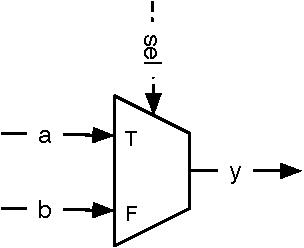
\includegraphics[scale=\scale]{../figures/mux}
\end{figure}
\shortlist{../code/mux.txt}
\begin{itemize}
\item So what?
\item Wait... What type is \code{a} and \code{b}?
\begin{itemize}
\item Can be any Chisel type!
\end{itemize}
\end{itemize}
\end{frame}

\begin{frame}[fragile]{Chisel has a Generic Multiplexer}
\begin{figure}
  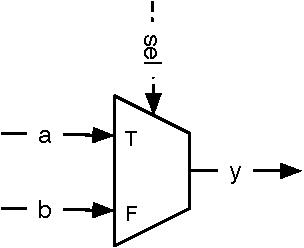
\includegraphics[scale=\scale]{../figures/mux}
\end{figure}
\shortlist{../code/mux.txt}
\begin{itemize}
\item SW people may not be impressed
\item They have generics since Java 1.5 in 2004
\begin{itemize}
\item \code{List<Flowers> != List<Cars>}
\end{itemize}
\end{itemize}
\end{frame}


\begin{frame}[fragile]{Generics in Hardware Construction}
\begin{itemize}
\item Chisel supports generic classes with type parameters
\item Write hardware generators independent of concrete type
\item This is a multiplexer \emph{generator}
\end{itemize}
\shortlist{../code/param_func.txt}
\end{frame}

\begin{frame}[fragile]{Put Generics Into Use}
\begin{itemize}
\item Let us implement a generic FIFO
\item Use the generic ready/valid interface from Chisel
\end{itemize}
\shortlist{../code/fifo_decoupled.txt}
\end{frame}

\begin{frame}[fragile]{Define the FIFO Interface}
\shortlist{../code/fifo_io.txt}
\begin{itemize}
\item We need enqueueing and dequeueing ports
\item Note the \code{Flipped}
\begin{itemize}
\item It switches the direction of ports
\item No more double definitions of an interface
\end{itemize}
\end{itemize}
\end{frame}

\begin{frame}[fragile]{But What FIFO Implementation?}
\begin{itemize}
\item Bubble FIFO (good for low data rate)
\item Double buffer FIFO (fast restart)
\item FIFO with memory and pointers (for larger buffers)
\begin{itemize}
\item Using flip-flops
\item Using on-chip memory
\end{itemize}
\item And some more...
\end{itemize}
\begin{itemize}
\item This calls for object-oriented \sout{programming} \emph{hardware construction}
\end{itemize}
\end{frame}

\begin{frame}[fragile]{Abstract Base Class and Concrete Extension}
\shortlist{../code/fifo_abstract.txt}
\begin{itemize}
\item May contain common code
\item Extend by concrete classes
\end{itemize}
\begin{chisel}
class BubbleFifo[T <: Data](gen: T, depth: Int) extends Fifo(gen: T, depth: Int) {
\end{chisel}
\end{frame}



\begin{frame}[fragile]{Select a Concrete FIFO Implementation}
\begin{itemize}
\item Decide at hardware generation
\item Can use all Scala/Java power for the decision
\begin{itemize}
\item Connect to a web service, get \sout{Google} Alphabet stock price, and decide on which to use ;-)
\item For sure a silly idea, but you see what is possible...
\item Developers may find clever use of the Scala/Java power
\item We could present a GUI to the user to select from
\end{itemize}
\item We use XML files parsed at hardware generation time
\item End of TCL, Python,... generated hardware
\end{itemize}
\end{frame}

\begin{frame}[fragile]{Binary to BCD Conversion for VHDL}
\begin{figure}
    \centering
    \includegraphics[scale=0.6]{JavaBCD}
\end{figure}
\end{frame}

\begin{frame}[fragile]{Java Program}
\begin{itemize}
\item Generates a VHDL table
\item The core code is:
\end{itemize}
\begin{chisel}
for (int i = 0; i < Math.pow(2, ADDRBITS); ++i) {
    int val = ((i/10)<<4) + i%10;
    // write out VHDL code for each line
\end{chisel}
\begin{itemize}
\item With all boilerplate 118 LoC
\end{itemize}
\end{frame}

\begin{frame}[fragile]{Chisel Version of Binary to BCD Conversion}
%\begin{chisel}
%  val array = new Array[Int](256)
%  for (i <- 0 to 99) {
%    array(i) = ((i/10)<<4) + i%10
%  }
%  val table = VecInit(array.map(_.U(8.W)))
%\end{chisel}
\begin{chisel}
  val table = Wire(Vec(100, UInt(8.W)))
  for (i <- 0 until 100) {
    table(i) := (((i/10)<<4) + i%10).U
  }
  val bcd = table(bin)
\end{chisel}
\begin{itemize}
\item Directly generates the hardware table as a \code{Vec}
\item At hardware construction time
\item In the same language
\end{itemize}
\end{frame}

\begin{frame}[fragile]{Use Functional Programming for Generators}
\shortlist{../code/fun_first.txt}
\shortlist{../code/fun_func_lit.txt}
\shortlist{../code/fun_reduce_tree.txt}
\begin{itemize}
\item This is a simple example
\item What about an arbiter tree with fair arbitration?
\end{itemize}
\end{frame}

\begin{frame}[fragile]{Functional Generation}
\begin{itemize}
\item Anonymous functions, called \emph{function literal}
\begin{chisel}
  (param) => function body
\end{chisel}
\item A function for a minimum search
\shortlist{../code/fun_min.txt}
\end{itemize}
\end{frame}

\begin{frame}[fragile]{Minimal Function with Index}
\begin{itemize}
\item Was the example for Tjark's heap sort
\shortlist{../code/fun_min2.txt}
\item We need an extra bundle to hold both values
\item A for loop is not so functional
\end{itemize}
\end{frame}

\begin{frame}[fragile]{We Can Use Tuples and zipWithIndex}
\begin{itemize}
\item \code{zipWithIndex} transforms the original sequence to a sequence of tuples
with second element is the index
\item Use \code{map} to translate from Scala \code{Int} to Chisel \code{UInt}
\item \code{reduce} does the minimum function, actually called 2 times (we could optimize this)
\shortlist{../code/fun_min3.txt}
\item The result is a Scala \code{Vector} and not a Chisel \code{Vec}
\end{itemize}
\end{frame}

\begin{frame}[fragile]{Solution with a Vec}
\begin{itemize}
\item Don't remember the details
\item But this results in a \code{Vec}
\shortlist{../code/fun_min4.txt}
\item
\item We should add a \code{reduceTree} to the Scala sequence version (\code{TraversableOnce})
\end{itemize}
\end{frame}

\begin{frame}[fragile]{An Arbiter}
\shortlist{../code/fun_arbiter.txt}
\end{frame}



\begin{frame}[fragile]{XXX}
\begin{itemize}
\item TODO: s4noc connection is part of the generator story
\item
\item
\end{itemize}
\end{frame}

\begin{frame}[fragile]{XXX}
\begin{itemize}
\item
\item
\item
\end{itemize}
\end{frame}



\begin{frame}[fragile]{Combinational (Truth) Table Generation}
\begin{chisel}
val arr = new Array[Bits](length)
for (i <- 0 until length) {
  arr(i) = ...
}
val rom = Vec[Bits](arr)
\end{chisel}
\begin{itemize}
\item Generate a table in a Scala array
\item Use that array as input for a Chisel \code{Vec}
\item Generates a logic table at hardware construction time
\end{itemize}
\end{frame}

\begin{frame}[fragile]{Ideas for Runtime Table Generation}
\begin{itemize}
\item Assembler in Scala/Java generates the boot ROM
\item Table with a \code{sin} function
\item Binary to BCD conversion
\item Schedule table for a TDM based network-on-chip
\item 
\item More ideas?
\end{itemize}
\end{frame}

\begin{frame}[fragile]{Memory}
\begin{chisel}
val mem = Mem(Bits(width = 8), size)

// write
when(wrEna) {
  mem(wrAddr) := wrData
}

// read
val rdAddrReg = Reg(next = rdAddr)
rdData := mem(rdAddrReg)
\end{chisel}
\begin{itemize}
\item Write is synchronous
\item Read can be asynchronous or synchronous
\item But there are no asynchronous memories in an FPGA
\end{itemize}
\end{frame}

\begin{frame}[fragile]{Factory Methods}
\begin{itemize}
\item Simpler component creation and use
\item Usage similar to built in components, such as \code{Mux}
\end{itemize}
\begin{chisel}
val myAdder = Adder(x, y)
\end{chisel}
\begin{itemize}
\item A little bit more work on component side
\item Define an \code{apply} method on the companion object that returns the component
\end{itemize}
\begin{chisel}
object Adder {
  def apply(a: UInt, b: UInt) = {
    val adder = Module(new Adder)
    adder.io.a := a
    adder.io.b := b
    adder.io.result
  }
}
\end{chisel}
\end{frame}

\begin{frame}[fragile]{Testing and Debugging}
\begin{itemize}
\item Nobody writes perfect code ;-)
\item We need a method to improve the code
\item In Java we can simply print the result:
\begin{itemize}
\item \code{println("42");}
\end{itemize}
\item What can we do in hardware?
\begin{itemize}
\item Describe the whole circuit and hope it works?
\item We can switch an LED on or off
\end{itemize}
\item We need some tools for \href{https://en.wikipedia.org/wiki/Debugging#/media/File:H96566k.jpg}{debugging}
\item Writing testers in Chisel
\end{itemize}
\end{frame}

\begin{frame}[fragile]{Testing with Chisel}
\begin{itemize}
\item Set input values with \code{poke}
\item Advance the simulation with \code{step}
\item Read the output values with \code{peek}
\item Compare the values with \code{expect}
\item Import following packages:
\shortlist{../code/test_import.txt}
\end{itemize}
\end{frame}

\begin{frame}[fragile]{Using \code{peek}, \code{poke}, and \code{expect}}
\begin{chisel}
// Set input values
poke(dut.io.a, 3)
poke(dut.io.b, 4)
// Execute one iteration
step(1)
// Print the result
val res = peek(dut.io.result)
println(res)

// Or compare against expected value
expect(dut.io.result, 7)
\end{chisel}
\end{frame}

\begin{frame}[fragile]{A Chisel Tester}
\begin{itemize}
\item Extends class \code{PeekPokeTester}
\item Has the device-under test (DUT) as parameter
\item Testing code can use all features of Scala
\end{itemize}
\begin{chisel}
class CounterTester(dut: Counter) extends PeekPokeTester(dut) {

  // Here comes the Chisel/Scala code
  // for the testing
}
\end{chisel}
\end{frame}

\begin{frame}[fragile]{Example DUT}
\begin{itemize}
\item A device-under test (DUT)
\shortlist{../code/test_dut.txt}
\end{itemize}
\end{frame}

\begin{frame}[fragile]{A Simple Tester}
\begin{itemize}
\item Just using \code{println} for manual inspection
\shortlist{../code/test_bench_simple.txt}
\end{itemize}
\end{frame}


\begin{frame}[fragile]{The Main Program for the Test}
\begin{itemize}
\item Extend an App and invoke the \code{iotesters} driver
\item With the DUT and the tester
\shortlist{../code/test_main_simple.txt}
\end{itemize}
\end{frame}

\begin{frame}[fragile]{A Real Tester}
\begin{itemize}
\item Poke values and \code{expect} some output
\shortlist{../code/test_bench.txt}
\end{itemize}
\end{frame}

\begin{frame}[fragile]{ScalaTest}
\begin{itemize}
\item Testing framework for Scala
\item \code{sbt} understands ScalaTest
\item Run all tests:
\code{sbt test}
\item When all \code{expect}s are ok, the test passes
\item A little bit funny syntax
\item Add library to \code{build.sbt}
\begin{chisel}
libraryDependencies += "org.scalatest" %% "scalatest" % "3.0.5" % "test"
\end{chisel}
\item Import ScalaTest library
\begin{chisel}
import org.scalatest._
\end{chisel}
\end{itemize}
\end{frame}

\begin{frame}[fragile]{ScalaTest Version of our Tester}
\shortlist{../code/scalatest_simple.txt}
\end{frame}

\begin{frame}[fragile]{Generating Waveforms}
\begin{itemize}
\item Waveforms are timing diagrams
\item Good to see many parallel signals and registers
\item Additional parameters: \code{"--generate-vcd-output", "on"}
\item IO signals and registers are dumped
\item Option \code{--debug} puts all wires into the dump
\item Generates a .vcd file
\item Viewing with GTKWave or ModelSim
\end{itemize}
\end{frame}


\begin{frame}[fragile]{Call the Tester}
\begin{itemize}
\item Using here ScalaTest
\item Note \code{Driver.execute}
\item Note \code{Array("--generate-vcd-output", "on")}
\end{itemize}
\begin{chisel}
class Count6WaveSpec extends
  FlatSpec with Matchers {
  
  "CountWave6 " should "pass" in {
    chisel3.iotesters.Driver.
    execute(Array("--generate-vcd-output", "on"),() => new Count6)
    { c => new Count6Wave(c) }
    should be (true)
  }
}
\end{chisel}
\end{frame}


\begin{frame}[fragile]{Test Driven Development (TDD)}
\begin{itemize}
\item Software development process
\begin{itemize}
\item Can we learn from SW development for HW design?
\end{itemize}
\item Writing the test first, then the implementation
\item Started with extreme programming
\begin{itemize}
\item Frequent releases
\item Accept change as part of the development
\end{itemize}
\item Not used in its pour form
\begin{itemize}
\item Writing all those tests is simply considerer too much work
\end{itemize}
\end{itemize}
\end{frame}


\begin{frame}[fragile]{Testing versus Debugging}
\begin{itemize}
\item Debugging is during code development
\item Waveform and println are easy tools for debugging
\item Debugging does not help for regression tests
\item Write small test cases for regression tests
\item Keeps your code base \emph{intact} when doing changes
\item Better confidence in changes not introducing new bugs
\end{itemize}
\end{frame}



\begin{frame}[fragile]{Summary}
\begin{itemize}
\item Chisel is a small language
\item Embedding it in Scala gives the power
\item We can write circuit generators
\item We can do co-simulation
\item We just scratched the surface
\end{itemize}
\end{frame}

\begin{frame}[fragile]{Links to the Examples}
\begin{itemize}
\item Example code
\end{itemize}
\begin{chisel}
https://github.com/schoeberl/chisel-examples.git
\end{chisel}
\begin{itemize}
\item Slides
\end{itemize}
\begin{chisel}
https://github.com/schoeberl/chisel-book.git
\end{chisel}
\end{frame}

\begin{frame}[fragile]{Feedback}
\begin{itemize}
\item Plans on using Chisel?
\item What went well?
\item What was not so good?
\item How can this Chisel course be improved?
\item
\item Would be happy to receive an email: \code{masca@dtu.dk}
\end{itemize}
\end{frame}

\begin{frame}[fragile]{Simulation Lab Session}
\begin{itemize}
\item Testing Hello World
\item Write test/verification code for a 5:1 multiplexer
\item A more interesting tester on an ALU accumulator
\item Project and DUT in GitHub lab1 and lab2
\item \url{https://github.com/chisel-uvm/class2020}
\item Extend it with ScalaTest (see Chisel book)
\end{itemize}
\end{frame}

\begin{frame}[fragile]{FPGA Lab Session}
\begin{itemize}
\item Run and explore the UART (serial port) example
\begin{itemize}
\item There is a make target that builds the UART hardware
\item \code{make uart}
\item It shall write some text out
\item You can observe it with a terminal (e.g., gtkterm)
\end{itemize}
\item Combine the UART with a blinking LED
\begin{itemize}
\item Write a `0' and `1' out on blink off and on
\item Best add the LEDs to \code{UartMain} and \code{uart\_top.vhdl}
\end{itemize}
\item Write repeated numbers 0--9 at maximum speed 
\end{itemize}
\end{frame}

\end{document}

%%%%%%%%%%%%%%%%
\begin{frame}[fragile]{Title}
\begin{chisel}
code
\end{chisel}
\begin{itemize}
\item xxx
\item xxx
\item xxx
\end{itemize}
\end{frame}

\begin{frame}[fragile]{Title}
\begin{itemize}
\item xxx
\item xxx
\item xxx
\item xxx
\item xxx
\end{itemize}
\end{frame}
%%%%%%%%%%%%%%%%

